\section{Approach}
\label{sec:approach}
\tool takes a code fragment from a user as input and searches code fragments from a software projects' code base to identify code fragments that are related to the user's input. Given an input code fragment, we first find all its similar methods in the code base, then trace back to the files that contain these similar methods and get other methods that co-ocur in the files as candidate related methods. Inside the candidate pool, for each candidate related method, we search for its similar methods from other files. Then we rank the candidate related methods by its number of similar ones and return the related methods by ranking. Figure \ref{fig:pipeline} illustrate the pipeline of finding related code fragments. 


\begin{figure}
	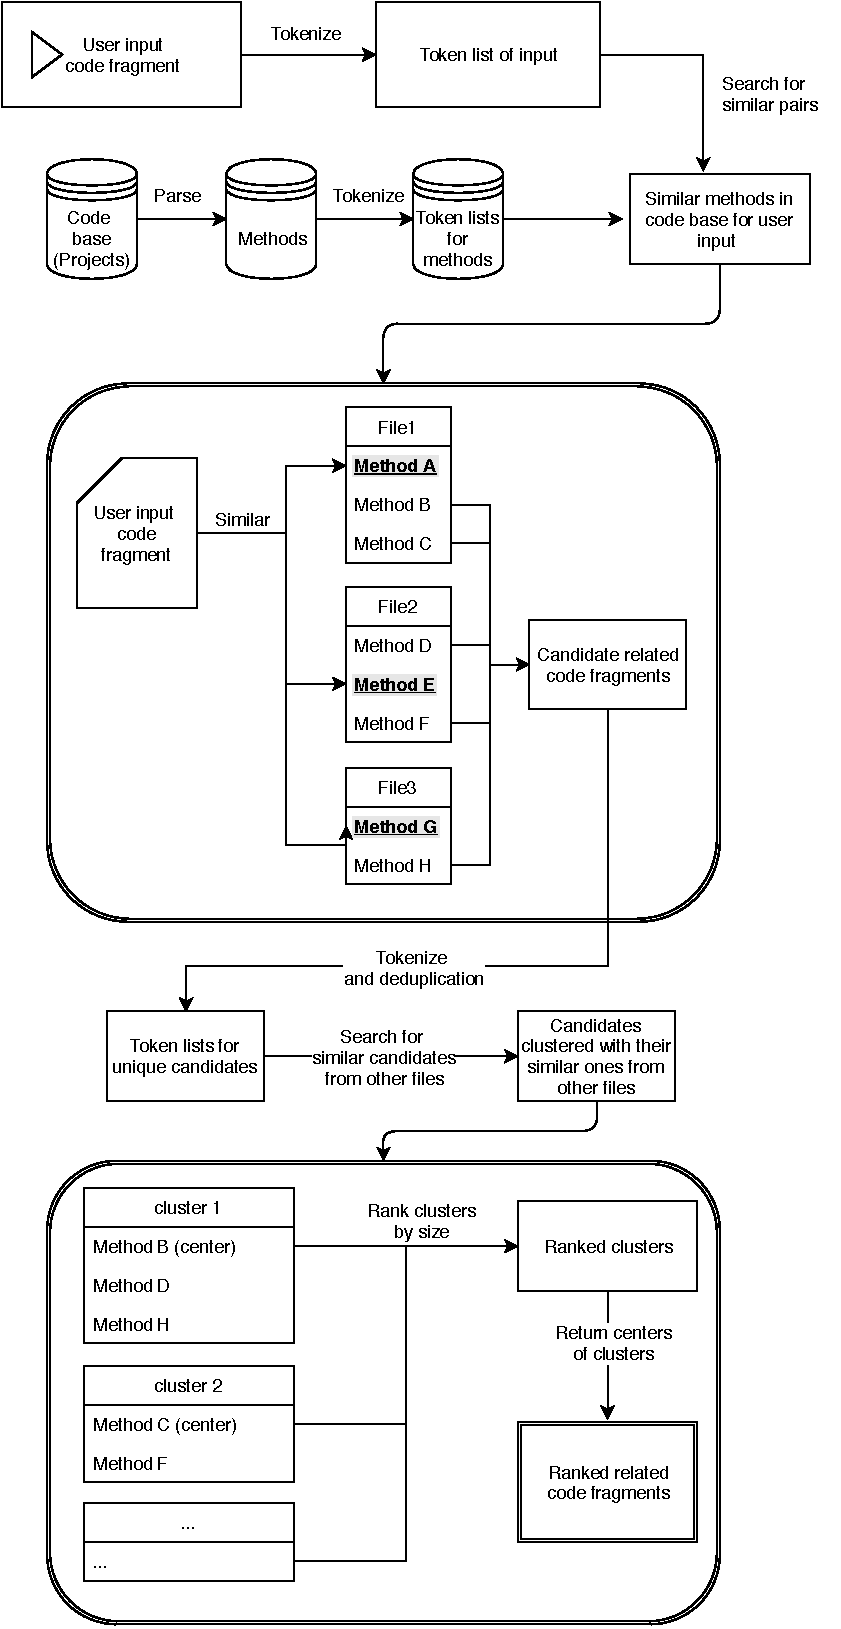
\includegraphics[width=\linewidth]{figures/pipeline.pdf}
	\caption{Pipeline of CodeAid}
	\label{fig:pipeline}
\end{figure}

\subsection{Retrieve similar methods}
\subsubsection{Parse code base projects}
For Java projects, our concept of code fragment is that of a method definition. For projects in the code base, we use Java parser to extract all methods defined in the \textit{.java} files.

\subsubsection{Tokenization}
Tokenization is the process of transforming a file into a bag of words. Tokenization involves removing comments, spaces, tabs and other special characters, identifying each individual word (token), and counting their frequency. During tokenization, tokens in the method are identified and their occurrences are counted, the result token list is in the format of 
\begin{lstlisting}
[(token1, freq1), (token2, freq2), 
(token3, freq3), ...)]
\end{lstlisting}
We tokenize both the input code fragment and all methods in the code base, in preparation for the next step of finding similar pairs.

\subsubsection{Search for similar methods}
For the input code fragment, we retrieve its similar counterparts from the code base. Here we use a code clone detection tool SoucererCC. By evaluating the scalability, execution time, recall and precision of SourcererCC, and comparing it to publicly available and state-of-the-art tools, SourcererCC has been shown to have both high recall and precision, and is able to scale to a large repository using a standard workstation. All of the above make SourcererCC a good candidate for this study. We set the similarity threshold to 70\% since it yields the best precision and recall on multiple clone benchmarks.

\subsection{Get candidate related code fragments}
After retrieving similar code fragments for the user input, we trace back to the files that contain these similar counterparts and get all other methods inside these files. As shown in Figure \ref{fig:pipeline}, the user input is similar to Method A in File 1, Method E in File 2, and Method G in File 3. File 1 also contains Method B and C, File 2 contains Method D and F, and Method H is File 3. Method B, C, D, F, and H will be our candidate for related code fragments, since they co-occur in the same file with similar methods to the user input. 

\subsection{Ranking}
\subsubsection{Search similar methods for each candidate}
For each candidate related method, we retrieve its token list again and find its similar method in other files. For example, Method B in File 1 is similar to Method D in File 2 and Method H in File 3, Method C in File 1 is similar to Method F in File 2. 

\subsubsection{Rank by number of similar methods}
After getting similar methods list for each candidate related method, we rank the candidates by its number of similar counterparts and return the ranked related method to the user.